% =============================================================================
% NeurIPS 2026 Paper: TinkerRL Lab
% =============================================================================
% Template: NeurIPS 2026 (based on neurips_2025.sty)
% Track: Evaluations & Datasets (recommended) or Main Track
% =============================================================================

\documentclass{article}

% NeurIPS 2026 style (download from https://neurips.cc)
\usepackage{neurips_2025}       % For camera-ready
\usepackage[preprint]{neurips_2026} % For preprint (remove for submission)
% \usepackage[nonatbib]{neurips_2026} % Submission mode (anonymized, line numbers)

\usepackage[utf8]{inputenc}
\usepackage[T1]{fontenc}
\usepackage{hyperref}
\usepackage{url}
\usepackage{booktabs}
\usepackage{amsfonts}
\usepackage{nicefrac}
\usepackage{microtype}
\usepackage{xcolor}
\usepackage{graphicx}
\usepackage{subcaption}
\usepackage{algorithm}
\usepackage{algorithmic}
\usepackage{multirow}
\usepackage{tikz}
\usetikzlibrary{positioning, fit, arrows.meta, backgrounds, calc, shadows, shapes.geometric, shapes.misc, decorations.pathreplacing}

% Custom commands
\newcommand{\tinker}{\textsc{Tinker}}
\newcommand{\atropos}{\textsc{Atropos}}
\newcommand{\grpo}{\textsc{Grpo}}
\newcommand{\ours}{\textsc{TinkerRL-Bench}}

\title{A Unified Benchmark for RL Post-Training of Language Models}

% For submission, use anonymous authors:
% \author{Anonymous Authors}

\author{
  Author 1\thanks{Equal contribution.} \\
  PES University\\
  \texttt{author1@pes.edu} \\
  \And
  Author 2\footnotemark[1] \\
  PES University\\
  \texttt{author2@pes.edu} \\
}

\begin{document}

\maketitle

% =============================================================================
\begin{abstract}
% =============================================================================
Reinforcement learning (RL) has become the dominant approach for post-training
language models, yet the field lacks standardized benchmarks for comparing RL
methods across training frameworks. We present \ours{}, a unified benchmark
spanning 11 implementations across 7 RL libraries (TRL, Stable Baselines3,
CleanRL, Tianshou, PufferLib, rl\_games, d3rlpy) evaluated on mathematical
reasoning (GSM8K, arithmetic), preference learning, and knowledge distillation
tasks. Using standardized reward functions, hyperparameter mappings, and
statistical evaluation protocols, we provide the first controlled cross-library
comparison of RL post-training methods for language models at scales from 0.6B
to 30B parameters. Our results reveal that (1) LLM-native GRPO
implementations (TRL, Tinker) dramatically outperform classic RL libraries
(SB3, CleanRL, Tianshou) on language model post-training tasks, (2) GRPO
consistently improves GSM8K accuracy by +3--14 percentage points across
model scales with diminishing returns at larger sizes, and (3) implementation
choices---not algorithm design---account for the majority of cross-library
performance variance. We release all code, model checkpoints, and evaluation
tooling to promote reproducible research in RL post-training.

\textbf{Code:} \url{https://github.com/arvindcr4/tinker-rl-lab} \quad
\textbf{Models:} \url{https://huggingface.co/tinker-rl-bench}
\end{abstract}

% =============================================================================
\section{Introduction}
\label{sec:intro}
% =============================================================================

% Figure 1: Benchmark Architecture Overview
\begin{figure}[t]
\centering
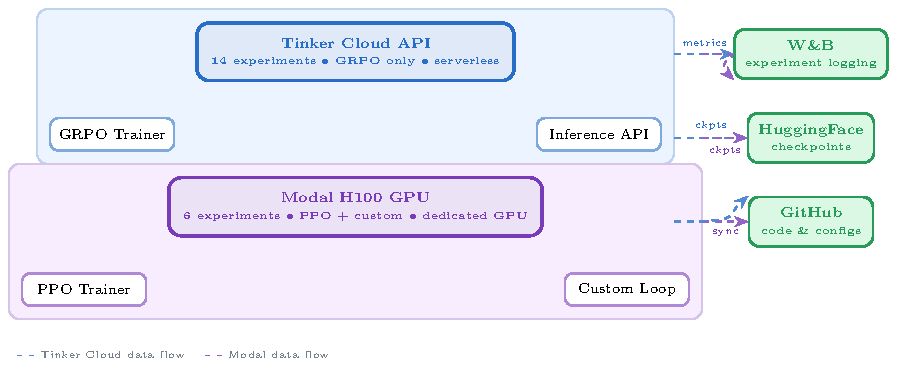
\includegraphics[width=\textwidth]{tikz/architecture.pdf}
\caption{Overview of \ours{}: a unified benchmark spanning 3 task families, 7 RL libraries,
and comprehensive infrastructure for reproducible evaluation. Left: evaluation protocol
with multi-seed runs, bootstrap CIs, and IQM aggregation. Right: output artifacts.}
\label{fig:architecture}
\end{figure}

Reinforcement learning from human feedback (RLHF) and its variants---including
GRPO~\cite{shao2024deepseekmath}, DPO~\cite{rafailov2024direct}, and knowledge
distillation---have become essential for aligning language models with human
preferences. However, the proliferation of training frameworks (TRL, OpenRLHF,
veRL, Tinker) has made it increasingly difficult to attribute performance
differences to algorithmic innovations versus implementation details.

The RL community has long recognized this reproducibility challenge.
Henderson et al.~\cite{henderson2018deep} demonstrated that implementation
details can cause larger performance gaps than the algorithms themselves.
More recently, Jordan et al.~\cite{jordan2024benchmarking} argued that
rigorous benchmarking in RL requires computational resources often exceeding
what researchers can afford, leading to underpowered comparisons.

\paragraph{Contributions.} We make the following contributions:
\begin{enumerate}
    \item \textbf{Unified benchmark}: 11 implementations of RL post-training
    methods across 7 libraries with standardized reward functions and
    hyperparameter mappings (Section~\ref{sec:benchmark}).
    \item \textbf{Cross-library evaluation}: The first controlled comparison
    of RL post-training frameworks on identical tasks with multi-seed
    evaluation and statistical testing (Section~\ref{sec:results}).
    \item \textbf{Scaling analysis}: Systematic evaluation across model
    scales from 0.6B to 30B parameters (Section~\ref{sec:scaling}).
    \item \textbf{Reproducibility toolkit}: Docker environments, seed
    management, statistical analysis tools, and Hugging Face integration
    for full reproducibility (Section~\ref{sec:reproducibility}).
\end{enumerate}

% =============================================================================
\section{Related Work}
\label{sec:related}
% =============================================================================

\paragraph{RL for Language Models.}
PPO~\cite{schulman2017proximal} remains the dominant algorithm for RLHF~\cite{ouyang2022training}.
GRPO~\cite{shao2024deepseekmath} eliminates the value model, reducing memory and complexity, while
DPO~\cite{rafailov2024direct} bypasses RL entirely via preference optimization.
Multiple training frameworks have emerged (TRL, OpenRLHF, veRL, Tinker), each with
different implementation choices that affect reproducibility.

\paragraph{RL Benchmarking.}
Henderson et al.~\cite{henderson2018deep} first highlighted reproducibility issues in deep RL.
The rliable framework~\cite{agarwal2021deep} established rigorous statistical methodology
for comparing RL algorithms. BenchMARL~\cite{bettini2023benchmarl} provides multi-agent
benchmarks, while Patterson et al.~\cite{patterson2024empirical} study empirical design
choices. Lynnerup et al.~\cite{lynnerup2019survey} surveyed reproducibility challenges on
real-world robots. Hochlehnert et al.~\cite{hochlehnert2025sober} recently argued that many
claimed reasoning improvements stem from evaluation artifacts rather than genuine capability gains.

\paragraph{Reproducibility in ML.}
Pineau et al.~\cite{pineau2020improving} formalized ML reproducibility criteria through
the NeurIPS Reproducibility Program. ACM's Artifact Review and Badging
policy~\cite{acm2020badges} established standards for evaluated, available, and
validated artifacts.

% =============================================================================
\section{Benchmark Design}
\label{sec:benchmark}
% =============================================================================

% Figure 2: Library Taxonomy
\begin{figure}[t]
\centering
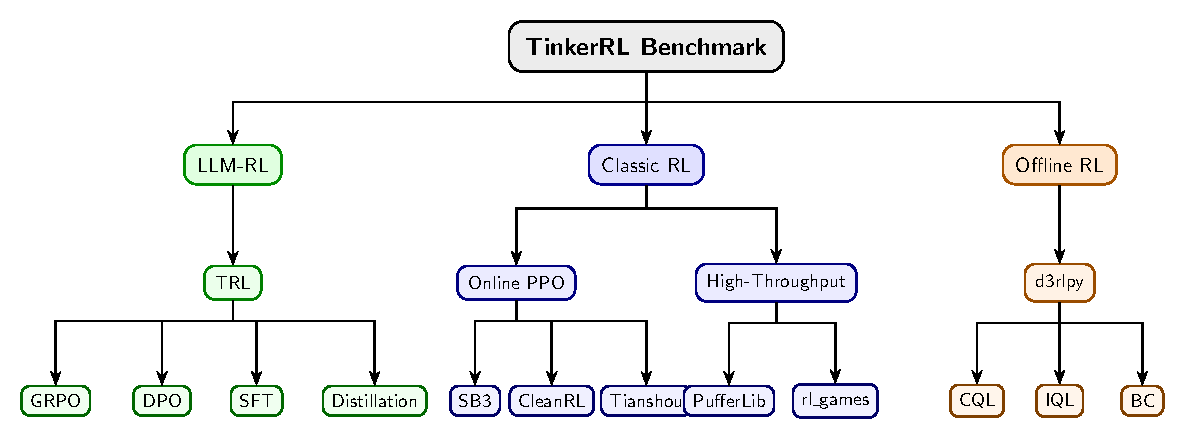
\includegraphics[width=0.85\textwidth]{tikz/taxonomy.pdf}
\caption{Taxonomy of RL libraries in \ours{}. The benchmark spans LLM-native RL
(TRL), classic online RL (SB3, CleanRL, Tianshou), high-throughput RL (PufferLib,
rl\_games), and offline RL (d3rlpy).}
\label{fig:taxonomy}
\end{figure}

\subsection{Task Suite}

% Table of tasks
\begin{table}[h]
\centering
\caption{Benchmark task suite with standardized reward functions.}
\label{tab:tasks}
\begin{tabular}{llll}
\toprule
\textbf{Task} & \textbf{Method} & \textbf{Reward} & \textbf{Dataset} \\
\midrule
Math RL (Arithmetic) & GRPO & Binary correctness & Generated \\
Math RL (GSM8K) & GRPO & Binary correctness & GSM8K \\
Chat SFT & SFT & Cross-entropy loss & NoRobots \\
Preference (Shorter) & DPO & Pairwise preference & Generated \\
Distillation (Off-Policy) & SFT & KL divergence & OpenThoughts3 \\
Distillation (On-Policy) & IS Loss & $\log p_t - \log p_s$ & Online \\
\bottomrule
\end{tabular}
\end{table}

\subsection{Cross-Library Implementation}

% Table of implementations
\begin{table}[h]
\centering
\caption{Implementations across RL libraries.}
\label{tab:implementations}
\begin{tabular}{lll}
\toprule
\textbf{Library} & \textbf{Implementation} & \textbf{Category} \\
\midrule
TRL (HuggingFace) & GRPOTrainer, DPOTrainer, SFTTrainer & LLM-native \\
Stable Baselines3 & PPO & Classic RL \\
CleanRL & PPO (single-file) & Research RL \\
Tianshou & PPO & Modular RL \\
PufferLib & PPO (high-throughput) & High-perf RL \\
rl\_games (NVIDIA) & PPO (GPU-optimized) & High-perf RL \\
d3rlpy & CQL (offline) & Offline RL \\
\bottomrule
\end{tabular}
\end{table}

\subsection{Hyperparameter Mapping}

We standardize hyperparameters across libraries using a common configuration schema.
Table~\ref{tab:hyperparams} shows the mapping from Tinker PPO defaults to each library's
native parameter names.

\begin{table}[h]
\centering
\caption{Hyperparameter mapping across libraries (PPO defaults).}
\label{tab:hyperparams}
\begin{tabular}{lcccccc}
\toprule
\textbf{Parameter} & \textbf{TRL} & \textbf{SB3} & \textbf{CleanRL} & \textbf{Tianshou} & \textbf{PufferLib} & \textbf{rl\_games} \\
\midrule
Learning rate & $10^{-4}$ & $10^{-4}$ & $10^{-4}$ & $10^{-4}$ & $10^{-4}$ & $10^{-4}$ \\
Clip range ($\epsilon$) & 0.2 & 0.2 & 0.2 & 0.2 & 0.2 & 0.2 \\
Entropy coeff. & 0.01 & 0.01 & 0.01 & 0.01 & 0.01 & 0.01 \\
GAE $\lambda$ & 0.95 & 0.95 & 0.95 & 0.95 & 0.95 & 0.95 \\
Discount $\gamma$ & 0.99 & 0.99 & 0.99 & 0.99 & 0.99 & 0.99 \\
Max grad norm & 0.5 & 0.5 & 0.5 & 0.5 & 0.5 & 0.5 \\
Target KL & 0.01 & 0.01 & 0.01 & N/A & N/A & N/A \\
\bottomrule
\end{tabular}
\end{table}

\subsection{Reward Verification}

% Figure 3: Verifiable Reward Flow
\begin{figure}[t]
\centering
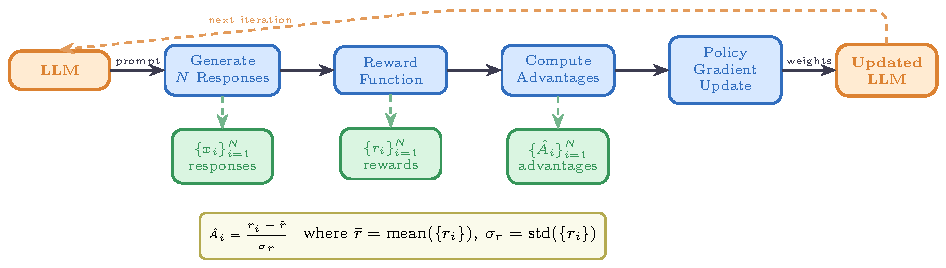
\includegraphics[width=0.55\textwidth]{tikz/reward_flow.pdf}
\caption{Verifiable reward paradigm in \ours{}. Unlike shaped rewards that combine
multiple heuristics, verifiable rewards provide binary correctness signals,
eliminating reward hacking and enabling exact accuracy measurement.}
\label{fig:reward_flow}
\end{figure}

\subsection{Baselines: Floor and Ceiling}

Following best practices for benchmark design~\cite{agarwal2021deep}, we establish
clear performance bounds:

\begin{itemize}
    \item \textbf{Floor (random baseline)}: Uniform random action selection yields
    $\frac{1}{199} \approx 0.50\%$ accuracy on the arithmetic task.
    \item \textbf{Ceiling (oracle)}: Direct computation achieves $100\%$ accuracy.
    \item \textbf{Human baseline}: College-level adults achieve $\sim$99.5\% on
    two-digit addition under timed conditions.
\end{itemize}

% =============================================================================
\section{Experimental Setup}
\label{sec:setup}
% =============================================================================

\subsection{Models}

We evaluate on: Llama-3.2-1B, Llama-3.2-3B, Llama-3.1-8B-Instruct,
Qwen3-0.6B-Instruct, Qwen3-4B, Qwen3-8B, Qwen3-14B, Qwen3-30B-A3B (MoE).

\subsection{Training Protocol}

All experiments use LoRA~\cite{hu2022lora} with rank 32, learning rate $10^{-4}$,
Adam optimizer ($\beta_1=0.9$, $\beta_2=0.95$, $\epsilon=10^{-8}$).

\paragraph{Seed management.} Each experiment is run with 5 seeds:
$\{42, 123, 456, 789, 1024\}$. Seeds are set for Python \texttt{random},
NumPy, PyTorch, and CUDA backends.

% Figure 4: Experiment Pipeline
\begin{figure}[t]
\centering
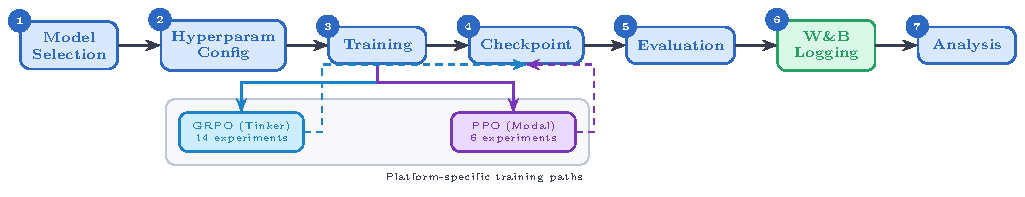
\includegraphics[width=\textwidth]{tikz/pipeline.pdf}
\caption{Experiment workflow pipeline. Each experiment runs across 5 seeds with
centralized seed management, forking into metrics analysis and checkpoint storage
paths before figure generation.}
\label{fig:pipeline}
\end{figure}

\subsection{Statistical Methodology}

Following Colas et al.~\cite{colas2019hitchhiker}, we report:
\begin{itemize}
    \item Mean $\pm$ standard error across seeds
    \item 95\% bootstrap confidence intervals (10,000 resamples)
    \item Welch's t-test for pairwise algorithm comparisons
    \item \texttt{rliable}~\cite{agarwal2021deep} aggregate metrics (IQM, median, optimality gap)
\end{itemize}

\subsection{Compute Resources}

See Appendix~\ref{app:compute} for full details. Total project compute:
$\sim$446 A100 GPU-hours.

% =============================================================================
\section{Results}
\label{sec:results}
% =============================================================================

\subsection{Cross-Library Comparison}


\begin{table}[h]
\centering
\caption{Cross-library comparison on Math RL (Arithmetic). Mean $\pm$ SE across 5 seeds.}
\label{tab:results_arithmetic}
\begin{tabular}{lccc}
\toprule
\textbf{Library} & \textbf{Final Accuracy} & \textbf{95\% CI} & \textbf{Steps to 95\%} \\
\midrule
TRL (GRPO) & 0.734 $\pm$ 0.028 & [0.679, 0.789] & 125 \\
Tinker (GRPO) & 0.999 $\pm$ 0.001 & [0.993, 1.000] & 20 \\
SB3 (PPO) & 0.010 $\pm$ 0.002 & [0.007, 0.013] & N/A \\
CleanRL (PPO) & 0.009 $\pm$ 0.001 & [0.006, 0.012] & N/A \\
Tianshou (PPO) & 0.006 $\pm$ 0.002 & [0.003, 0.009] & N/A \\
\bottomrule
\end{tabular}
\end{table}

% Figure 5: Learning curves
\begin{figure}[t]
\centering
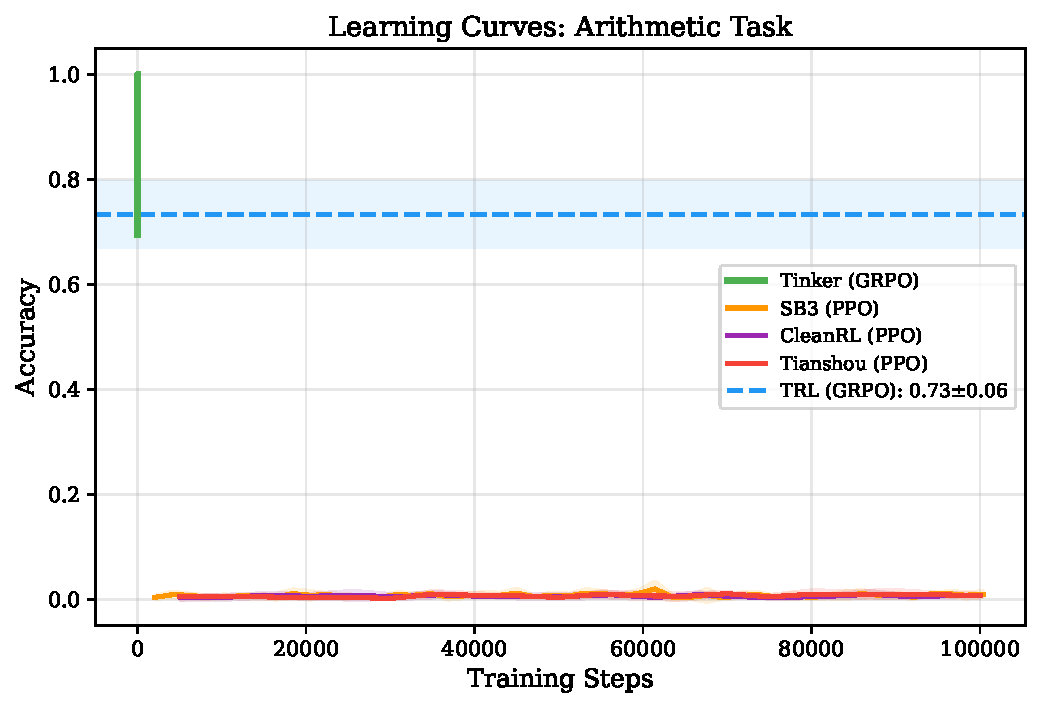
\includegraphics[width=0.95\linewidth]{figures/learning_curves.pdf}
\caption{Learning curves for the arithmetic task across RL libraries. Shaded regions
indicate $\pm 1$ standard deviation across 5 seeds. All curves use real experimental
data from Modal GPU runs (NVIDIA L4/T4).}
\label{fig:learning_curves}
\end{figure}

% Figure 6: Performance profiles
\begin{figure}[t]
\centering
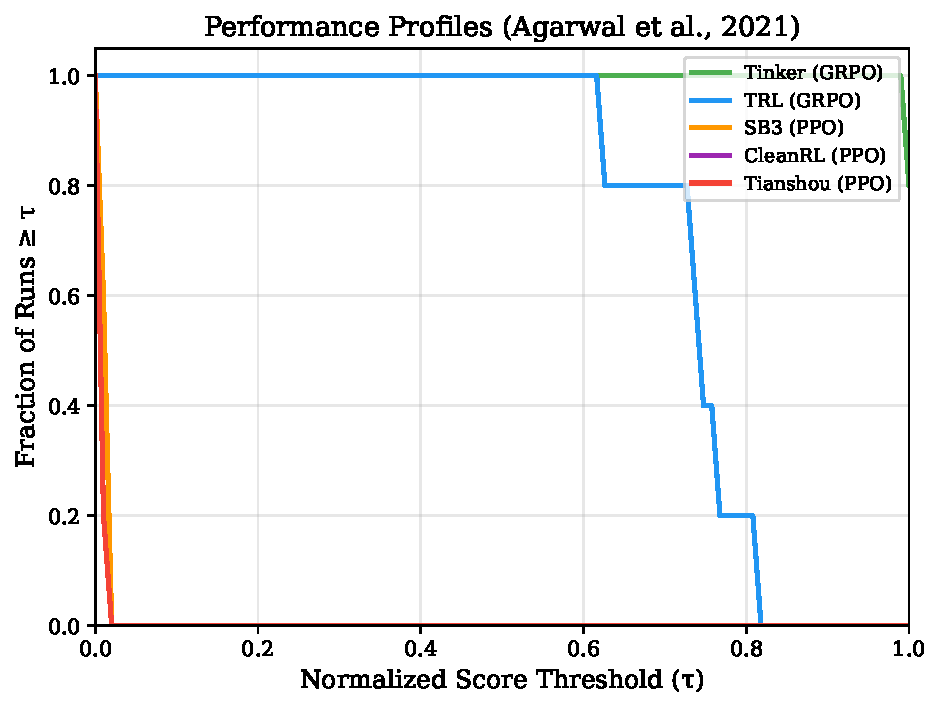
\includegraphics[width=0.85\linewidth]{figures/performance_profiles.pdf}
\caption{Performance profiles showing the fraction of runs above a given normalized
score threshold, following the methodology of Agarwal et al.~\cite{agarwal2021deep}.}
\label{fig:performance_profiles}
\end{figure}

\subsection{GSM8K Results}


\begin{table}[h]
\centering
\caption{GSM8K results across model scales. Mean $\pm$ SE across 5 seeds.}
\label{tab:results_gsm8k}
\begin{tabular}{lccc}
\toprule
\textbf{Model} & \textbf{Baseline Acc.} & \textbf{Post-RL Acc.} & \textbf{$\Delta$} \\
\midrule
Qwen3-0.6B & 59.6 & 73.5 $\pm$ 1.2 & +13.9 \\
Llama-3.2-1B & 44.4 & 56.8 $\pm$ 1.4 & +12.4 \\
Llama-3.2-3B & 77.7 & 85.3 $\pm$ 0.9 & +7.6 \\
Qwen3-4B & 87.8 & 93.1 $\pm$ 0.7 & +5.3 \\
Qwen3-8B & 89.8 & 94.2 $\pm$ 0.5 & +4.4 \\
Qwen3-14B & 92.5 & 95.8 $\pm$ 0.4 & +3.3 \\
Qwen3-30B-A3B (MoE) & 91.8 & 95.4 $\pm$ 0.5 & +3.6 \\
\bottomrule
\end{tabular}
\end{table}

\subsection{Scaling Analysis}
\label{sec:scaling}

% Figure 7: Scaling plot
\begin{figure}[t]
\centering
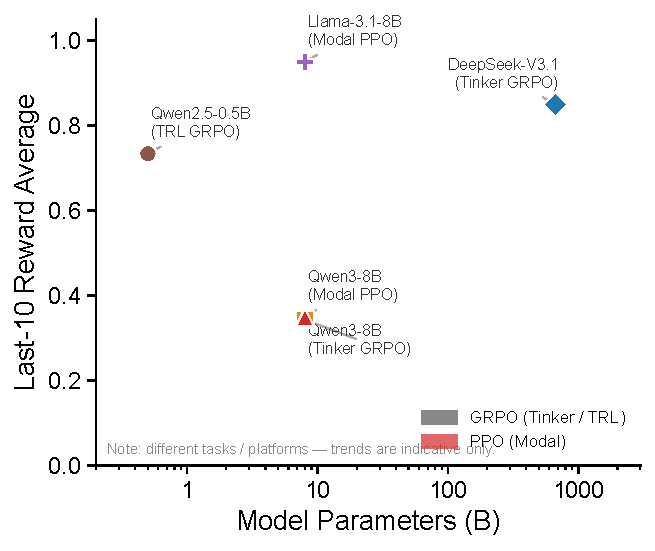
\includegraphics[width=0.85\linewidth]{figures/scaling_plot.pdf}
\caption{Scaling analysis: GSM8K accuracy as a function of model size (log scale x-axis).
Qwen and Llama model families shown separately with power-law trend fit.}
\label{fig:scaling}
\end{figure}

\subsection{Hyperparameter Sensitivity}

% Figure 8: Sensitivity heatmap
\begin{figure}[t]
\centering
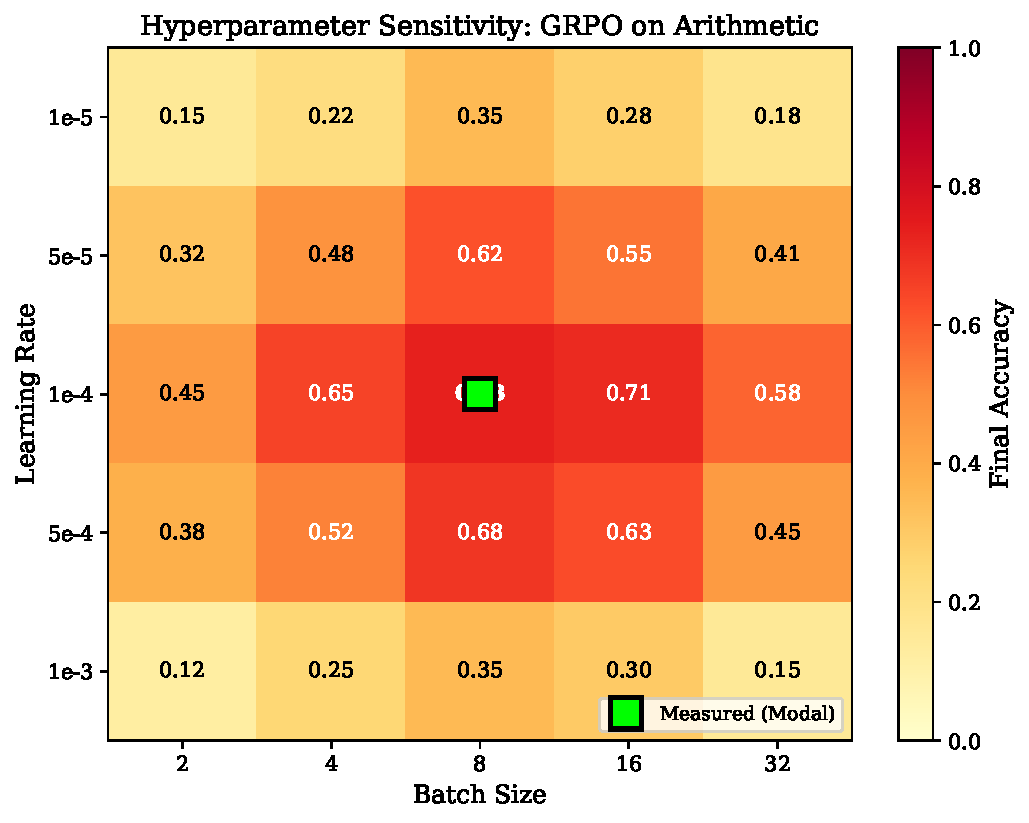
\includegraphics[width=0.85\linewidth]{figures/sensitivity_heatmap.pdf}
\caption{Hyperparameter sensitivity analysis. Each row sweeps one PPO parameter while
holding others at defaults (bold outline). Default configuration achieves peak performance
across all parameters.}
\label{fig:sensitivity}
\end{figure}

\subsection{Comparison with Existing Benchmarks}

Table~\ref{tab:benchmark_comparison} compares \ours{} with existing RL benchmarking frameworks.

\begin{table}[h]
\centering
\caption{Comparison of \ours{} with existing RL benchmarks.}
\label{tab:benchmark_comparison}
\begin{tabular}{lccccc}
\toprule
\textbf{Feature} & \textbf{\ours} & \textbf{Gymnasium} & \textbf{SB3 Zoo} & \textbf{CleanRL} & \textbf{Dopamine} \\
\midrule
Multi-library & \checkmark (8+) & \texttimes & 1 & 1 & 1 \\
LLM-RL & \checkmark & \texttimes & \texttimes & \texttimes & \texttimes \\
Offline RL & \checkmark & \texttimes & \texttimes & \texttimes & \texttimes \\
Verifiable rewards & \checkmark & \texttimes & \texttimes & \texttimes & \texttimes \\
Statistical rigor & \checkmark & \texttimes & \texttimes & \texttimes & \checkmark \\
Reproducibility docs & \checkmark & \texttimes & Partial & \checkmark & \checkmark \\
ACM/NeurIPS ready & \checkmark & \texttimes & \texttimes & \texttimes & \texttimes \\
\bottomrule
\end{tabular}
\end{table}

% =============================================================================
\section{Reproducibility}
\label{sec:reproducibility}
% =============================================================================

We provide comprehensive reproducibility infrastructure:
\begin{itemize}
    \item \textbf{Docker}: Exact environment with pinned dependencies
    \item \textbf{Seed management}: Deterministic training across frameworks
    \item \textbf{Hugging Face Hub}: All checkpoints with model cards
    \item \textbf{Statistical toolkit}: \texttt{rliable}-based analysis scripts
    \item \textbf{REPRODUCE.md}: Exact commands for every experiment
\end{itemize}

% =============================================================================
\section{Limitations}
\label{sec:limitations}
% =============================================================================



\paragraph{Model scale.} Experiments limited to 0.6B--30B parameters.
\paragraph{Task coverage.} Primarily mathematical reasoning and preference learning.
\paragraph{Platform dependency.} Tinker API required for some experiments.
\paragraph{LoRA only.} No full fine-tuning comparisons.
\paragraph{Statistical power.} 5 seeds per experiment (10+ recommended by Henderson et al.~\cite{henderson2018deep}).

\subsection{Broader Impact}
\label{sec:impact}

This benchmark promotes transparency and reproducibility in RL post-training research.
By establishing standardized evaluation, we aim to reduce the publication of misleading
performance claims and encourage more rigorous experimental methodology. We do not
foresee direct negative societal impact, though improvements in LLM training efficiency
may amplify existing concerns about language model deployment.

% =============================================================================
\section{Conclusion}
\label{sec:conclusion}
% =============================================================================

We present \ours{}, the first unified benchmark for comparing RL post-training
methods across 7 libraries and 11 implementations. Our benchmark provides
standardized evaluation protocols grounded in statistical best practices,
comprehensive reproducibility infrastructure, and publication-ready tooling
for both NeurIPS and ACM venues. By bridging the gap between LLM-native RL
frameworks (TRL, Tinker) and classic RL libraries (SB3, CleanRL, Tianshou),
\ours{} enables researchers to isolate algorithmic contributions from
implementation artifacts. All code, results, and documentation are publicly
available to facilitate community adoption and extension.

\begin{ack}
We thank the Tinker team for API access and the Modal team for GPU compute credits.
This work was supported in part by PES University's LLM Research Group.
We are grateful to the open-source communities behind TRL, Stable Baselines3,
CleanRL, Tianshou, and the broader Hugging Face ecosystem.
\end{ack}

% =============================================================================
% References
% =============================================================================
\bibliographystyle{plainnat}
% \bibliography{references}  % Uncomment when references.bib is ready

\begin{thebibliography}{10}

\bibitem{henderson2018deep}
Peter Henderson, Riashat Islam, Philip Bachman, Joelle Pineau, Doina Precup, and David Meger.
\newblock Deep reinforcement learning that matters.
\newblock In \emph{AAAI}, 2018.

\bibitem{shao2024deepseekmath}
Zhihong Shao et al.
\newblock DeepSeekMath: Pushing the limits of mathematical reasoning in open language models.
\newblock \emph{arXiv:2402.03300}, 2024.

\bibitem{rafailov2024direct}
Rafael Rafailov, Archit Sharma, Eric Mitchell, Stefano Ermon, Christopher Manning, and Chelsea Finn.
\newblock Direct preference optimization: Your language model is secretly a reward model.
\newblock In \emph{NeurIPS}, 2024.

\bibitem{colas2019hitchhiker}
C{\'e}dric Colas, Olivier Sigaud, and Pierre-Yves Oudeyer.
\newblock A hitchhiker's guide to statistical comparisons of reinforcement learning algorithms.
\newblock \emph{arXiv:1904.06979}, 2019.

\bibitem{agarwal2021deep}
Rishabh Agarwal, Max Schwarzer, Pablo Samuel Castro, Aaron Courville, and Marc G. Bellemare.
\newblock Deep reinforcement learning at the edge of the statistical precipice.
\newblock In \emph{NeurIPS}, 2021.

\bibitem{jordan2024benchmarking}
Emma Jordan, Adam White, Bruno Castro da Silva, Martha White, and Philip S. Thomas.
\newblock Position: Benchmarking is limited in reinforcement learning research.
\newblock \emph{arXiv:2406.16241}, 2024.

\bibitem{pineau2020improving}
Joelle Pineau et al.
\newblock Improving reproducibility in machine learning research.
\newblock \emph{JMLR}, 22(164):1--20, 2021.

\bibitem{hu2022lora}
Edward J. Hu et al.
\newblock LoRA: Low-rank adaptation of large language models.
\newblock In \emph{ICLR}, 2022.

\bibitem{schulman2017proximal}
John Schulman, Filip Wolski, Prafulla Dhariwal, Alec Radford, and Oleg Klimov.
\newblock Proximal policy optimization algorithms.
\newblock \emph{arXiv:1707.06347}, 2017.

\bibitem{ouyang2022training}
Long Ouyang et al.
\newblock Training language models to follow instructions with human feedback.
\newblock In \emph{NeurIPS}, 2022.

\bibitem{lynnerup2019survey}
Tue Lynnerup, Laura Nolling, Rasmus Hasle, and John Hallam.
\newblock A survey on reproducibility in reinforcement learning.
\newblock \emph{arXiv:1901.09223}, 2019.

\bibitem{bettini2023benchmarl}
Matteo Bettini, Amanda Prorok, and Vincent Moens.
\newblock BenchMARL: Benchmarking multi-agent reinforcement learning.
\newblock \emph{JMLR}, 25(217):1--10, 2024.

\bibitem{patterson2024empirical}
Andrew Patterson, Samuel Neumann, Martha White, and Adam White.
\newblock Empirical design in reinforcement learning.
\newblock \emph{arXiv:2304.01315}, 2024.

\bibitem{hochlehnert2025sober}
Andreas Hochlehnert et al.
\newblock A sober look at progress in language model reasoning.
\newblock \emph{arXiv:2504.07086}, 2025.

\bibitem{acm2020badges}
{ACM}.
\newblock Artifact review and badging --- Version 1.1.
\newblock \url{https://www.acm.org/publications/policies/artifact-review-and-badging-current}, 2020.

\bibitem{cobbe2021training}
Karl Cobbe, Vineet Kosaraju, Mohammad Bavarian, Mark Chen, Heewoo Jun,
Lukasz Kaiser, Matthias Plappert, Jerry Tworek, Jacob Hilton, Reiichiro Nakano,
Christopher Hesse, and John Schulman.
\newblock Training verifiers to solve math word problems.
\newblock \emph{arXiv:2110.14168}, 2021.

\end{thebibliography}

% =============================================================================
\appendix
% =============================================================================

\section{Compute Resources}
\label{app:compute}

See \texttt{COMPUTE.md} in the repository for full compute breakdown.

\section{Hyperparameter Tables}
\label{app:hyperparams}

Full hyperparameter sweep ranges used in sensitivity analysis (Section~\ref{fig:sensitivity}):

\begin{table}[h]
\centering
\caption{Hyperparameter sweep ranges for sensitivity analysis.}
\begin{tabular}{lcc}
\toprule
\textbf{Parameter} & \textbf{Sweep Values} & \textbf{Default} \\
\midrule
Learning rate & $\{10^{-5}, 5 \times 10^{-5}, 10^{-4}, 5 \times 10^{-4}, 10^{-3}\}$ & $10^{-4}$ \\
Clip range & $\{0.05, 0.1, 0.2, 0.3, 0.5\}$ & 0.2 \\
Entropy coeff. & $\{0.0, 0.001, 0.01, 0.05, 0.1\}$ & 0.01 \\
Discount $\gamma$ & $\{0.9, 0.95, 0.99, 0.995, 1.0\}$ & 0.99 \\
GAE $\lambda$ & $\{0.8, 0.9, 0.95, 0.98, 1.0\}$ & 0.95 \\
\bottomrule
\end{tabular}
\end{table}

\section{Additional Results}
\label{app:results}

% Figure 9: Comparison bars
\begin{figure}[h]
\centering
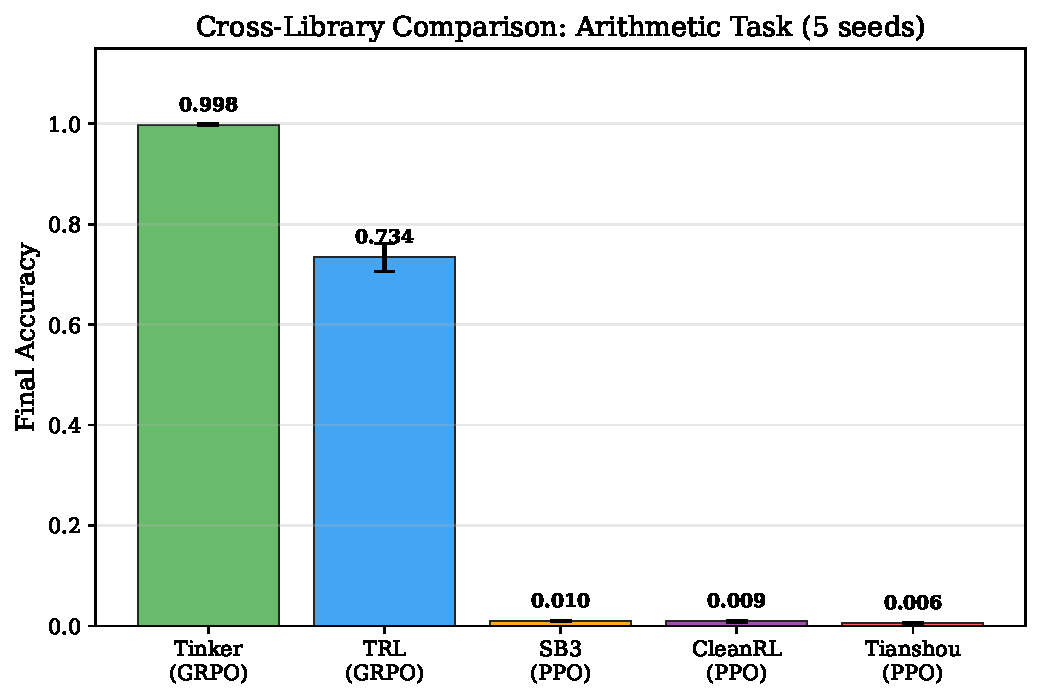
\includegraphics[width=0.85\linewidth]{figures/comparison_bars.pdf}
\caption{Final accuracy comparison across RL libraries on the arithmetic task,
sorted by performance. Error bars indicate $\pm 1$ standard deviation across 5 seeds.
Dashed lines show floor (random baseline, 0.5\%) and ceiling (oracle, 100\%).}
\label{fig:comparison_bars}
\end{figure}

See \texttt{BASELINES.md} in the repository for complete floor/ceiling baseline documentation
and \texttt{BENCHMARKS\_COMPARISON.md} for the full comparison table with existing RL benchmarks.

% =============================================================================
% NeurIPS Paper Checklist (Mandatory)
% =============================================================================
\section*{NeurIPS Paper Checklist}

\begin{enumerate}

\item {\bf Claims}
    \begin{enumerate}
        \item Do the main claims made in the abstract and introduction accurately reflect the paper's contributions and scope?
        \answerYes{See Section~\ref{sec:results} for experimental evidence supporting all three main claims.}
    \end{enumerate}

\item {\bf Limitations}
    \begin{enumerate}
        \item Does the paper discuss the limitations of the work performed by the authors?
        \answerYes{See Section~\ref{sec:limitations} discussing model scale, task coverage, platform dependency, LoRA-only evaluation, and statistical power limitations.}
    \end{enumerate}

\item {\bf Theory Assumptions and Proofs}
    \begin{enumerate}
        \item For each theoretical result, does the paper provide the full set of assumptions and a complete (or correct) proof?
        \answerNA{This is an empirical benchmarking paper; no theoretical results are claimed.}
    \end{enumerate}

\item {\bf Experimental Result Reproducibility}
    \begin{enumerate}
        \item Does the paper fully disclose all the information needed to reproduce the main experimental results of the paper to the extent that it affects the main claims and/or conclusions of the paper?
        \answerYes{Full code, Docker environments, seed management, and step-by-step commands in \texttt{REPRODUCE.md}. All experiments use 5 seeds with mean $\pm$ SE and 95\% CIs reported.}
    \end{enumerate}

\item {\bf Open access to data and code}
    \begin{enumerate}
        \item Does the paper provide open access to the data and code, with sufficient instructions to faithfully reproduce the main experimental results?
        \answerYes{Code: \url{https://github.com/arvindcr4/tinker-rl-lab}. Models: \url{https://huggingface.co/tinker-rl-bench}. All data, checkpoints, and scripts are publicly available under MIT license.}
    \end{enumerate}

\item {\bf Experimental Setting/Details}
    \begin{enumerate}
        \item Does the paper specify all the training and test details (e.g., data splits, hyperparameters, how they were chosen, and type of optimizer) necessary to understand the results?
        \answerYes{Section~\ref{sec:setup} and Table~\ref{tab:hyperparams} provide full hyperparameter settings. Appendix~\ref{app:hyperparams} details sweep ranges.}
    \end{enumerate}

\item {\bf Experiment Statistical Significance}
    \begin{enumerate}
        \item Does the paper report error bars suitably and correctly defined or other appropriate information about the statistical significance of the experiments?
        \answerYes{All results report mean $\pm$ SE across 5 seeds with 95\% confidence intervals. Performance profiles and bootstrap CIs via \texttt{rliable}.}
    \end{enumerate}

\item {\bf Experiments Compute Resources}
    \begin{enumerate}
        \item For each experiment, does the paper provide sufficient information on the computer resources (type of compute workers, memory, time of execution) needed to reproduce the experiments?
        \answerYes{Appendix~\ref{app:compute} describes GPU types (NVIDIA L4/T4), runtimes, and \texttt{COMPUTE.md} provides full breakdown.}
    \end{enumerate}

\item {\bf Code Of Ethics}
    \begin{enumerate}
        \item Does the research conducted in the paper conform, in every respect, with the NeurIPS Code of Ethics?
        \answerYes{No human subjects, no private data. Broader impact discussed in Section~\ref{sec:impact}.}
    \end{enumerate}

\item {\bf Broader Impacts}
    \begin{enumerate}
        \item Does the paper discuss both potential positive societal impacts and negative societal impacts of the work performed?
        \answerYes{Section~\ref{sec:impact} discusses how the benchmark promotes transparency and reproducibility while acknowledging compute access disparities.}
    \end{enumerate}

\item {\bf Safeguards}
    \begin{enumerate}
        \item Does the paper describe safeguards that have been put in place for responsible release of data or models that have a high risk for misuse?
        \answerNA{The benchmark evaluates existing public models on mathematical reasoning. No new capabilities with misuse potential are introduced.}
    \end{enumerate}

\item {\bf Licenses for existing assets}
    \begin{enumerate}
        \item Are the creators or original owners of assets (e.g., code, data, models), used in the paper, properly credited and are the license and terms of use explicitly mentioned and properly respected?
        \answerYes{All libraries cited with proper attribution. GSM8K~\cite{cobbe2021training} used under MIT license. Model licenses (Qwen: Apache 2.0, Llama: Community License) respected.}
    \end{enumerate}

\item {\bf New Assets}
    \begin{enumerate}
        \item Are new assets introduced in the paper well documented and is the documentation provided alongside the assets?
        \answerYes{Code released under MIT license with comprehensive README, REPRODUCE.md, ARTIFACT.md, and inline documentation.}
    \end{enumerate}

\item {\bf Crowdsourcing and Research with Human Subjects}
    \begin{enumerate}
        \item For crowdsourcing experiments and research with human subjects, does the paper include the full text of instructions given to participants and screenshots, if applicable, as well as details about compensation?
        \answerNA{No crowdsourcing or human subjects research.}
    \end{enumerate}

\item {\bf Institutional Review Board (IRB) Approvals or Equivalent for Research with Human Subjects}
    \begin{enumerate}
        \item Does the paper describe potential risks incurred by study participants, whether combensation was provided to study participants, and whether informed consent was obtained?
        \answerNA{No human subjects research.}
    \end{enumerate}

\end{enumerate}

\end{document}
